\section{Exact laws and ties}\label{sec:aging}

Recall the model. After its first step the walk switches
direction at step $k\ge2$ with probability $c/k$, independently of the past,
where $0<c<2$. So the walk switches less and less often, and the expected
number of switches in $N$ steps is $c(H_N-1)$, which is about $c\log N$. With
a fair first step, $A_N/N$ converges in law to
$\mathrm{Beta}(c,c)$~\cite[Example~1.1 and Theorem~1.4]{ds2007},
\cite[Theorem~2]{ev2018}. At finite $N$ the first step
matters. We first give one exact law behind all the ties, then fix the first
step, pass to $d$ states, and return to the fair first step.

As in Section~\ref{sec:notation}, $\Prob_+$ is the law given $X_1=+1$ and
$X_N$ is the last step. A path is a sequence
$x\in\{\pm1\}^N$, and it switches at time $t\ge2$ if $x_t\ne x_{t-1}$. Step
$k\ge2$ contributes the factor $c/k$ to the probability of a path if the path
switches there, and $1-c/k$ otherwise. So relative to no switch, a switch at
time $t$ multiplies the probability of a path by the odds
\[
 \omega_t=\frac{c/t}{1-c/t}=\frac{c}{t-c}\qquad(t\ge2),
\]
and
\begin{equation}\label{eq:aging-path}
 \Prob_+(X=x)=\prod_{k=2}^N\Bigl(1-\frac ck\Bigr)\prod_{t:\,x_t\ne x_{t-1}}\omega_t
 \qquad(x_1=+1).
\end{equation}
Each $\omega_t$ is positive and continuous on $(0,2)$, increases strictly in
$c$, and tends to $0$ as $c\downarrow0$.

\subsection{Drawing afresh or repeating}\label{sec:aging-urn}

All the exact laws of this section come from one chain, which works for every
weight. Fix $d\ge2$ and $\theta>0$, and let $Y_1,Y_2,\dots$ be the following
chain on $\{1,\dots,d\}$. At step $t\ge1$, with probability
\[
 f_t=\frac{d\theta}{d\theta+t-1}
\]
the state $Y_t$ is drawn afresh, uniformly from the $d$ states, and otherwise
$Y_t=Y_{t-1}$ (so $Y_1$ is uniform, since $f_1=1$). In other words, at
step $t\ge2$ the chain moves to each other state with probability
$\theta/(d\theta+t-1)$. This is the mechanism of the conservative random walk
of Engl\"ander and Volkov~\cite{ev2022}, who redraw a direction in
$\mathbb Z^d$ with probability $p_n$ and study recurrence and scaling limits.
Let $M_T$ be the vector of visit counts of $Y_1,\dots,Y_T$, and write
$x^{(m)}=x(x+1)\cdots(x+m-1)$.

\begin{proposition}[fresh or repeat]\label{prop:aging-urn}
For every $T\ge1$, every composition $m$ of $T$ into $d$ nonnegative parts and
every state $j$,
\begin{equation}\label{eq:aging-urn}
 \Prob(M_T=m,\,Y_T=j)=\frac{m_j}{T}\,Q_T(m),\qquad
 Q_T(m)=\frac{T!}{(d\theta)^{(T)}}\prod_{i=1}^d\frac{\theta^{(m_i)}}{m_i!} .
\end{equation}
So $M_T$ has the law $Q_T$ of the counts in P\'olya's urn with $d$ colors and
initial weight $\theta$ on each color. For $d=2$ and even $T\ge2$,
\begin{equation}\label{eq:aging-urn-ratio}
 \frac{\Prob(M_T=(T/2,T/2))}{\Prob(M_T=(T,0))}
 =\binom{T}{T/2}\prod_{i=0}^{T/2-1}\frac{\theta+i}{\theta+T/2+i},
\end{equation}
which increases strictly in $\theta$ and equals $1$ exactly at $\theta=1$.
\end{proposition}

In words, the chain repeats its last state where the urn repeats a uniformly
chosen earlier draw, and at each fixed time this makes no difference to the
counts or to the last state. Figure~\ref{fig:aging} shows the law below, at
and above the tie.

\begin{figure}[t]
\centering
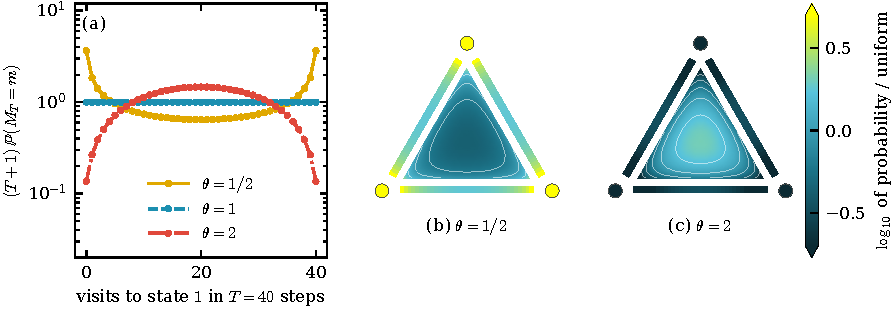
\includegraphics[width=\textwidth]{figures/aging}
\caption{The exact law~\eqref{eq:aging-urn} of the counts of the chain that
draws afresh or repeats. (a) Two states and $T=40$, as a multiple of the
uniform law. The law is flat at $\theta=1$, the ends are the most likely points
for $\theta=\frac12$, and the center is for $\theta=2$. (b), (c) Three states
and $T=36$ on the simplex of visit fractions, colored by the probability of a
count vector relative to the uniform law. The triangle holds the count vectors
that use all 3 states, the bands hold those that use 2, and the disks are
those that use 1. The thin lines are level lines. For $\theta=\frac12$ a corner is
$9.6$ times as likely as under the uniform law and the center $0.43$ times.
For $\theta=2$ the numbers are $0.035$ and $2.1$.}
\label{fig:aging}
\end{figure}

\begin{proof}
We use induction on $T$. For $T=1$ both sides of~\eqref{eq:aging-urn} are
$\frac1d$ when $m=e_j$ and $0$ otherwise. Let $T\ge2$ and suppose
\eqref{eq:aging-urn} holds for $T-1$. If $m_j=0$ both sides vanish. Otherwise
put $m'=m-e_j$. Summing~\eqref{eq:aging-urn} over the last state gives
$\Prob(M_{T-1}=m')=Q_{T-1}(m')$. A fresh draw gives $j$ with probability
$\frac1d$ whatever the last state was, and a repeat gives $j$ only when the
last state was $j$ (this is why the induction carries the last state along
with the counts). So
\[
 \Prob(M_T=m,\,Y_T=j)
 =\frac{f_T}{d}\,Q_{T-1}(m')+(1-f_T)\,\frac{m_j-1}{T-1}\,Q_{T-1}(m')
 =\frac{\theta+m_j-1}{d\theta+T-1}\,Q_{T-1}(m') .
\]
On the other hand
$Q_T(m)=Q_{T-1}(m')\cdot\frac{T}{m_j}\cdot\frac{\theta+m_j-1}{d\theta+T-1}$ by
the definition of $Q_T$. This gives~\eqref{eq:aging-urn}. Summing over $j$
gives $\Prob(M_T=m)=Q_T(m)$, and the ratio~\eqref{eq:aging-urn-ratio} is
$Q_T(T/2,T/2)/Q_T(T,0)$ with
$\theta^{(T)}=\theta^{(T/2)}(\theta+T/2)^{(T/2)}$. Each factor
$(\theta+i)/(\theta+T/2+i)$ increases strictly in $\theta$, and at
$\theta=1$ the product is $(T/2)!^2/T!$.
\end{proof}

The law of the counts alone is known. Dietz, Lippitt and
Sethuraman~\cite[Theorem~2.18]{dls2023} show that the moments of the limit
law of the chains of~\cite{ds2007} are occupation probabilities at finite $N$
of a second chain. In the case of a Dirichlet limit that second chain is
$Y$, with the uniform law in the role of their $\mu$ and $d\theta$ in the role
of their $\theta$. The limit is then the Dirichlet law with every parameter
$\theta$~\cite[Theorem~1.4]{ds2007}, and its moments give $Q_T$.
Engl\"ander and Volkov work it out in Chapter~7 of their
March 18, 2024 draft~\cite{ev2024}. For 2 states and an integer weight $\theta$
they prove~\eqref{eq:aging-urn}, with the last state, for every
$T$~\draftloc{Theorem~7.2, pp.~138--139}, and they credit this result to E.~Crane.
What the proposition adds is the joint law with the last state for $d\ge3$
states, and for a weight $\theta$ that is not an integer. As $T\to\infty$,
\eqref{eq:aging-urn} turns into the joint limit of the fractions of time and
the current state found by Bouguet and Cloez~\cite[Proposition~4.1]{bc2018},
in which the Dirichlet law is size-biased by the coordinate of the current
state.

\begin{remark}\label{rem:aging-feller}
Here is another way to see the law of the counts in
Proposition~\ref{prop:aging-urn} (but not the joint law with the last state).
The fresh draws
cut $Y_1,\dots,Y_T$ into runs, and each run gets a uniform state. The urn can
be run in the same way, as a Chinese restaurant process in which each table
gets a uniform color. There a table is opened with the same probabilities
$f_t$. The lengths of the runs are the spacings between the successes of
independent trials with success probabilities $f_t$. It is a classical
fact (the Feller coupling, see~\cite{abt2003}) that the multiset of these spacings has
the same law as the multiset of the table sizes (the two ordered lists do not).
The proof in~\draftloc{Section~7.4}, like
Proposition~\ref{prop:aging-urn}, instead goes through the last state. We
checked~\eqref{eq:aging-urn} in exact arithmetic for 4 values of $\theta$,
with $T\le7$ for $d=2,3$ and $T\le5$ for $d=4$
(\texttt{verify\_aging\_urn.py}).
\end{remark}

\subsection{A fixed first step}

Here the walk starts with a step $+1$.

\begin{proposition}[2 states, fixed first step]\label{prop:aging-two}
Let $N\ge2$ and let the first step be $+1$.
\begin{enumerate}[(a)]
\item At $c=1$, for $1\le s\le N$,
\[
 \Prob_+(A_N=s,\,X_N=+1)=\frac{s-1}{N(N-1)},\qquad
 \Prob_+(A_N=s,\,X_N=-1)=\frac{N-s}{N(N-1)}.
\]
So $A_N$ is uniform on $\{1,\dots,N\}$.
\item For $1\le s\le N-1$ the ratio $\Prob_+(A_N=s)/\Prob_+(A_N=N)$ increases
strictly in $c\in(0,2)$, and it equals $1$ exactly at $c=1$.
\end{enumerate}
\end{proposition}

For $c<1$ the end $N$ is the most likely value of $A_N$, and for $c>1$ it is
the least likely of the values $1,\dots,N$ (the value $0$ has probability
$0$).

\begin{proof}
(a) At $c=1$, the shifted chain $Y_t=X_{t+1}$ is the chain of
Proposition~\ref{prop:aging-urn} with $d=2$, $\theta=1$ and uniform first
state. Apply~\eqref{eq:aging-urn} at $T=N-1$ with counts $(s-1,N-s)$,
where $Q_{N-1}=1/N$, then sum over the last state.

(b) We write the ratio as a sum over paths. Only the path with every step
$+1$ has $A_N=N$, and it never switches. So $\Prob_+(A_N=N)$ is the first
product in~\eqref{eq:aging-path}, and dividing by it leaves
\begin{equation}\label{eq:aging-ratio}
 \frac{\Prob_+(A_N=s)}{\Prob_+(A_N=N)}
 =\sum_{x}\ \prod_{t:\,x_t\ne x_{t-1}}\omega_t ,
\end{equation}
where the sum is over the paths $x$ with $x_1=+1$ and $s$ steps equal to
$+1$. For example, for $N=3$ and $s=2$ the paths are $(+,+,-)$ and $(+,-,+)$,
and the ratio is $\omega_3+\omega_2\omega_3$. For $1\le s\le N-1$ there is
such a path, and each of them switches at least once. So the right side is a
sum of products of the $\omega_t$ with at least one factor each. Each
$\omega_t$ is positive and increases strictly in $c$, so the sum does too. By
(a) it equals $1$ at $c=1$.
\end{proof}

After a shift of one step, part (a) is the exercise
in~\cite[Section~3.1, footnote~1]{evw2020}. That footnote also says that the fact
can be related to P\'olya urns (the authors credit M.~Bal\'azs) and that a
more general connection of their model with P\'olya urns will appear in a
later paper.
That connection is developed in Chapter~7 of the dated draft, and after the same
shift part (a), with the last state, is~\draftloc{Claim~7.1}. So part (a)
is not new. What we add for
2 states is part (b), and the count law also follows
from~\cite[Theorem~2.18]{dls2023} (Section~\ref{sec:aging-urn}). Both parts of
Proposition~\ref{prop:aging-two} are also proved in Lean
(Section~\ref{sec:verify}).

\subsection{\texorpdfstring{$d$}{d} states}

The same thing happens for a chain on $d$ states that leaves its current
state for each other state at the same aging rate. Fix $d\ge2$ and $\theta$
with $0<\theta<d/(d-1)$. The chain $X_1,X_2,\dots$ on $\{1,\dots,d\}$ starts at
$X_1=1$. At step $k\ge2$ it moves to each of the other $d-1$ states with
probability $\theta/(k+d-2)$, and it stays with probability
$1-(d-1)\theta/(k+d-2)$. The condition on $\theta$ says that the probability
of staying is positive at every step $k\ge2$. Let
$L_N=(L_N(1),\dots,L_N(d))$ be the vector of visit counts, namely
$L_N(i)=\#\{k\le N:X_k=i\}$. Its values are the compositions
$n=(n_1,\dots,n_d)$ of $N$ into $d$ nonnegative parts with $n_1\ge1$. There
are $\binom{N+d-2}{d-1}$ of them (subtract one from $n_1$). The corner
$Ne_1$, where $e_i$ is the $i$-th unit vector, is the count vector of the
chain that never moves.

For such chains Dietz and Sethuraman~\cite[Theorem~1.4]{ds2007} proved that
the fractions of time converge in law to the Dirichlet law with every
parameter $\theta$, which is uniform on the simplex exactly at $\theta=1$.
Our step $k$ uses their transition matrix at time $n=k+d-2$, and the two
agree for $n\ge d+1$. Both chains redraw a uniform state with probability
$d\theta/n$. After the first common redraw they agree, so their fractions of
time have the same limit. At
$\theta=1$, part~(a) of the theorem below is an exact finite-$N$ form of this
limit.

\begin{theorem}[$d$ states]\label{thm:aging-d}
Let $d\ge2$, $0<\theta<d/(d-1)$ and $N\ge2$.
\begin{enumerate}[(a)]
\item At $\theta=1$, for every count vector $n$ and every state $j$,
\begin{equation}\label{eq:aging-d}
 \Prob(L_N=n,\,X_N=j)=\frac{n_j-\mathbf 1\{j=1\}}{(N-1)\binom{N+d-2}{d-1}} .
\end{equation}
So $L_N$ is uniform on its $\binom{N+d-2}{d-1}$ values, the corner included.
\item For every count vector $n\ne Ne_1$ the ratio $\Prob(L_N=n)/\Prob(L_N=Ne_1)$
increases strictly in $\theta$, and it equals $1$ exactly at $\theta=1$.
\end{enumerate}
\end{theorem}

In words, at $\theta=1$, given the counts, the
last state is distributed as the state at a uniformly chosen one of the steps
$2,\dots,N$ (the forced first visit to state $1$ is left out).
Below $\theta=1$ the corner is the most likely count vector, and above it the corner
is the least likely.

\begin{proof}
(a) At $\theta=1$, $X_2$ is uniform and $Y_t=X_{t+1}$ is the chain
of Proposition~\ref{prop:aging-urn}. Its count vector is $L_N-e_1$, and
$Q_{N-1}=1/\binom{N+d-2}{d-1}$. Formula~\eqref{eq:aging-urn} gives
\eqref{eq:aging-d}, and summing over $j$ gives the uniform law.

(b) A path $x\in\{1,\dots,d\}^N$ with $x_1=1$ has probability
$\prod_{k=2}^N\bigl(1-\frac{(d-1)\theta}{k+d-2}\bigr)$ times the product of
the odds
\[
 \omega^{(d)}_t=\frac{\theta/(t+d-2)}{1-(d-1)\theta/(t+d-2)}
 =\frac{\theta}{t+d-2-(d-1)\theta}
\]
over the times $t\ge2$ with $x_t\ne x_{t-1}$. The denominator is positive and
decreases in $\theta$, so each $\omega^{(d)}_t$ increases strictly in
$\theta$. Only the constant path has counts $Ne_1$. So
$\Prob(L_N=n)/\Prob(L_N=Ne_1)$ is the sum of the products of the odds over
the paths with counts $n$. For a count vector $n\ne Ne_1$ there is such a path, and
each of them moves at least once. Hence the ratio increases strictly in
$\theta$, and by (a) it equals $1$ at $\theta=1$.
\end{proof}

\begin{remark}\label{rem:aging-d}
For $d=2$ the chain switches at step $k$ with probability $\theta/k$, so
Theorem~\ref{thm:aging-d} with $\theta=c$ is
Proposition~\ref{prop:aging-two}, and~\eqref{eq:aging-d} reads
$(s-1)/(N(N-1))$ for $j=1$ and $n=(s,N-s)$.

By Proposition~\ref{prop:aging-urn}, $(L_N-e_1,X_N)$ has the law of
the counts and last color of $N-1$ draws from P\'olya's urn with one ball of
each color. This is an identity at each fixed time, not an identity of path
laws. For example, with $d=2$ and $N=4$ the chain path $1,1,2,2$ has
probability $1/8$, while the urn draws $1,2,2$ have probability $1/12$.
For 2 states Engl\"ander and Volkov call this relation
mimicking~\draftloc{Definition~7.1 and Lemma~7.1}, and they show with an
example of 3 steps that the coin-turning walk and the urn have different
path laws~\draftloc{Example~7.1}. Also, at $\theta=1$ the chain moves at
step $k$ with probability $(d-1)/(k+d-2)$, independently over $k$. This is
the probability that customer $k$ opens a new table in the Chinese restaurant
process with parameter $d-1$. So the expected number of moves in $N$ steps at
the tie is $\sum_{k=2}^N\frac{d-1}{k+d-2}=(d-1)\log N+O(1)$, which has the
same order, $\log N$, as the number of turns at the crossing from the corners
to the center for $d$ directions and runs of geometric length
(Section~\ref{sec:prior}).

We checked~\eqref{eq:aging-d}, and the strict ordering in (b) along the 5
values $\theta=\frac12,\frac9{10},1,\frac{11}{10},\frac54$, in exact
rational arithmetic for $d=2,3,4$ and $2\le N\le8$
(\texttt{verify\_aging.py}).
\end{remark}

\subsection{A fair first step}

We return to 2 states and let the first step be fair. Then both ends can be
reached, and $E_N=\Prob(A_N=N)=\frac12\prod_{k=2}^N(1-c/k)$. Changing the sign
of every step preserves the law of the walk and sends $A_N$ to $N-A_N$. So
\begin{equation}\label{eq:aging-fair}
 \Prob(A_N=s)=\tfrac12\bigl(\Prob_+(A_N=s)+\Prob_+(A_N=N-s)\bigr),\qquad
 E_N=\tfrac12\Prob_+(A_N=N),
\end{equation}
since $\Prob_+(A_N=0)=0$.

\begin{proposition}[fair first step]\label{prop:aging-fair}
Let $N\ge2$ and $1\le s\le N-1$, with a fair first step.
\begin{enumerate}[(a)]
\item At $c=1$, $\Prob(A_N=s)=\frac1N$ and $E_N=\frac1{2N}$.
\item The ratio $\Prob(A_N=s)/E_N$ is continuous and strictly increasing in
$c\in(0,2)$. It tends to $0$ as $c\downarrow0$ and equals $2$ at $c=1$. So
there is exactly one $c$ in $(0,2)$ with $\Prob(A_N=s)=E_N$, and it is less
than $1$.
\end{enumerate}
\end{proposition}

For even $N$ we write $c_N$ for the crossing in (b) with $s=h=N/2$, so that
$C_N=E_N$ exactly at $c=c_N$. In words, at $c=1$ every interior point still has
probability $\frac1N$, and the two ends share the probability $\frac1N$ that
the fixed start gave to one end.
Engl\"ander and Volkov give related fair-start formulas for switch
probabilities $1/(n+a)$~\draftloc{Section~5.7, p.~76}. We derive (a) from the
symmetry identity~\eqref{eq:aging-fair} instead.

\begin{proof}
(a) This follows from~\eqref{eq:aging-fair} and
Proposition~\ref{prop:aging-two}(a). (b) By~\eqref{eq:aging-fair} the ratio
is the sum of the right sides of~\eqref{eq:aging-ratio} for $s$ and for
$N-s$. Both are finite sums of products of at least one $\omega_t$. So the
ratio is continuous and strictly increasing, and it tends to $0$ as
$c\downarrow0$. By (a) it equals $2$ at $c=1$. Hence it equals $1$ exactly
once, at some $c<1$.
\end{proof}

How far below $1$ is $c_N$? The end is of order $N^{-c}$ and the center is of
order $1/N$, so they meet when $N^{1-c}$ is about $2$.

\begin{proposition}[the fair-start crossing]\label{prop:aging-expansion}
For even $N\to\infty$,
\[
 c_N=1-\frac{\log2}{\log N+\gamma+2-2\log2}+O\bigl((\log N)^{-3}\bigr),
\]
where $\gamma$ is Euler's constant.
\end{proposition}

\paragraph{Idea of the proof.}
A monotonicity argument first traps $c_N$ within $O(1/\log N)$ of $1$, so an expansion at $c=1$
applies. The end is explicit, namely
$E_N=\Gamma(N+1-c)/(2\Gamma(2-c)\Gamma(N+1))$, which is
$N^{-c}/(2\Gamma(2-c))$ with relative error $O(1/N)$. For the center we prove
a local limit theorem with a rate, namely $NC_N=d_c+O(\sqrt{\log N/N})$ uniformly
for $c\in[c^{(3)},1]$, where $c^{(3)}=(9-\sqrt{57})/2\approx0.725$ and $d_c=4^{1-c}/\mathrm B(c,c)$ is the density of
$\mathrm{Beta}(c,c)$ at $\frac12$. So
$\log(C_N/E_N)=(c-1)\log N+\Theta(c)+O(\sqrt{\log N/N})$ with
$\Theta(c)=\log(2\Gamma(2-c)d_c)$. Here $\Theta(1)=\log2$ and
$\Theta'(1)=\gamma+2-2\log2$, and solving for the zero gives the expansion.
The proof is in Appendix~\ref{app:aging}. There $C_N$ is an average of
explicit numbers over the law of the time of the $h$-th step $+1$
(Lemma~\ref{lem:D-average}). The local limit theorem comes from a coupling of
the walk with the chain of Proposition~\ref{prop:aging-urn} with $d=2$ and
$\theta=c$, whose counts are a mixture of binomial laws with a
$\mathrm{Beta}(c,c)$ parameter (Proposition~\ref{prop:D-llt}).

The error term decays only like $(\log N)^{-3}$, but the expansion is
already accurate at moderate $N$. The computed crossing at $N=200$ is
$c_{200}=0.8925$, against $0.8932$ from the expansion without its error term. The constant in
the error term is not computed.
